\documentclass[12pt]{article}

%\pagestyle{empty} 
\usepackage{amsmath}
\usepackage{algpseudocode}
\usepackage{algorithm}
\usepackage[english]{babel}
\usepackage{amsthm}
\usepackage{amssymb}
\usepackage{color}
\usepackage{graphicx}
\usepackage{epsfig}
\usepackage{tikz}

\newcommand{\vs}{\vspace{2mm}}
\newcommand{\ls}{\vspace{5mm}} 

\newcommand{\ms}{\vspace{3mm}}
\newcommand{\bc}{\begin{center}}
\newcommand{\ec}{\end{center}}
\newcommand{\sm}{\small}
\newcommand{\hs}{\hspace{10mm}}
\newcommand{\ha}{\hspace{1mm}}
\newcommand{\bo}{\rule{2mm}{3mm}}
\textheight=680pt
\textwidth=460pt
\hoffset=-50pt
\voffset=-50pt
%\topmargin=-0.5in
%\textheight=10in
%\oddsidemargin=0.125in
%\evensidemargin=0.125in
%\textwidth=7.5in
\begin{document}
\bc\ 
 { \bf Homework  4 (50 points)}  Due: October 04, 2024 11:59 pm\\
 { \bf COMPSCI 733: Advanced Algorithms and Designs } \\ 
 { \bf Benzon Carlitos Salazar (salazarbc24@uww.edu) } 
\ec\
\ls\

\noindent{\bf Documentation:} (5 points)
Type your solutions using Latex \\
(www.overleaf.com or https://www.latex-project.org/ ). Submit your solutions (pdf is enough)  to Canvas. 

\vs\
\noindent{\bf Problem 1: } (25 points)
\vs\

\begin{itemize}

\item[(a)] Let $G = (V, E)$ be an undirected simple graph with finite number of vertices. Prove that 
\[ 2 |E| = \sum_{v \in V} deg(v), \]
where $deg(v)$ is the number of edges incident with the vertex $v$.
 \ls\

\begin{proof}   
Let $G = (V, E)$ be an undirected simple graph, where $V$ is the set of vertices and $E$ is the set of edges. For each vertex $v \in V$, let $\deg(v)$ denote the degree of vertex $v$, which is the number of edges incident to $v$.

Now, consider the sum of the degrees of all vertices in the graph:
\[
\sum_{v \in V} \deg(v)
\]
Each edge in the graph contributes exactly two to the total sum of degrees, since every edge is incident to exactly two vertices in an undirected graph. That is, for each edge $e = (u, v) \in E$, the vertices $u$ and $v$ both have their degrees increased by 1 due to the edge $e$.

Thus, the sum of the degrees of all the vertices is twice the number of edges in the graph:
\[
\sum_{v \in V} \deg(v) = 2|E|.
\]
\end{proof}

\item[(b)] Let $G = (V, E)$ be an undirected simple connected  graph. Prove that  the BFS algorithms discussed in the class runs in time $O(|V|+|E|),$ if the graph is given by the adjacency list
representation. (Hint: Use the Part (a) result.)

\begin{proof}
BFS starts at a source vertex and explores all vertices and edges in the graph. The graph is represented using an adjacency list, where for each vertex $v$, we store a list of its adjacent vertices. We now analyze the running time of BFS:
\begin{itemize}
    \item[1.] \textbf{Initialization:} BFS initializes data structures such as the queue, distances, and predecessors. This takes $O(|V|)$ time because we have to initialize each vertex individually.

    \item[2.]  \textbf{Exploring Vertices:} Each vertex is enqueued and dequeued exactly once during the BFS traversal. Since there are $|V|$ vertices, this step takes $O(|V|)$ time.

    \item[3.]  \textbf{Exploring Edges:} For each vertex $v \in V$, BFS iterates over all of its neighbors, i.e., all vertices adjacent to $v$. The time to explore the neighbors of a vertex $v$ is proportional to the degree of $v$, denoted $\deg(v)$. Therefore, the total time to explore all neighbors of all vertices is
    \[
    O\left( \sum_{v \in V} \deg(v) \right).
    \]
    By the result from Part (a), we know that
    \[
    \sum_{v \in V} \deg(v) = 2|E|.
    \]
    Thus, the time spent exploring edges is $O(2|E|) = O(|E|)$.

    \item[4.] \textbf{Total Time Complexity:} The total time is the sum of the time spent on initialization, vertex exploration, and edge exploration. Hence, the overall time complexity of BFS is
    \[
    O(|V| + |E|).
    \]
\end{itemize}
\end{proof}


\item[(c)] What is the complexity for Part (b) if an adjacency matrix is used?

\begin{proof}
When the graph is represented using an adjacency matrix, the BFS algorithm works as follows:
\begin{itemize}
    \item[1.] \textbf{Initialization:}  Initializing the BFS queue and distance array takes $O(|V|)$, since there are $|V|$ vertices.
    
    \item[2.] \textbf{Exploring Vertices:}  Each vertex is enqueued and dequeued exactly once during BFS, which takes $O(|V|)$ time.
    
    \item[3.] \textbf{Exploring Edges:}  For each vertex $v \in V$, BFS must check whether there is an edge between $v$ and each other vertex $u \in V$. Since the graph is represented by an adjacency matrix, this requires scanning through the entire row of the matrix corresponding to $v$, which takes $O(|V|)$ time for each vertex. Therefore, the total time for edge exploration is
    \[
    O(|V|) \times |V| = O(|V|^2).
    \]
    
    \item[4.] \textbf{Total Time Complexity:}  The overall time complexity is the sum of the time spent on initialization, vertex exploration, and edge exploration, which gives
    \[
    O(|V| + |V| + |V|^2) = O(|V|^2).
    \]
\end{itemize}
\end{proof}

\item[(d)] A sequence of integers $d_1, d_2, \ldots , d_n$ is called graphic if it is the degree sequence of a simple undirected graph. Using basic graph properties including Problem 1a, determine whether each of these sequences is graphic. For those that are, draw a graph having the given sequence. For those that are not, provide  reasons for why no graph has such a sequence. 
\vs\

\noindent{(1) 5, 4, 3, 2, 1, 0 }\\
(2) 6, 5, 4, 3, 2, 1 \\
(3) 2, 2, 2, 2, 2, 2 \\
(4) 3, 3, 3, 2, 2, 2 \\
(5) 3, 3, 2, 2, 2, 2 \\
(6) 1, 1, 1, 1, 1, 1 \\
(7) 5, 3, 3, 3, 3, 3 \\
(8) 5, 5, 4, 3, 2, 1 \\

\textbf{Answer:}

\begin{itemize}
    \item[(1)] {5, 4, 3, 2, 1, 0} \\
    \textbf{Sum of degrees}: \( 5 + 4 + 3 + 2 + 1 + 0 = 15 \) (odd number). \\
    \textbf{Conclusion}: This sequence is \textbf{not graphic}, because the sum of the degrees is odd, violating the Handshaking Lemma.
    \item[(2)] {6, 5, 4, 3, 2, 1} \\
    \textbf{Sum of degrees}: \( 6 + 5 + 4 + 3 + 2 + 1 = 21 \) (odd number). \\
    \textbf{Conclusion}: This sequence is \textbf{not graphic}, because the sum of the degrees is odd, violating the Handshaking Lemma.
    \item[(3)] {2, 2, 2, 2, 2, 2} \\
    \textbf{Sum of degrees}: \( 2 + 2 + 2 + 2 + 2 + 2 = 12 \) (even number). \\
    \textbf{Havel-Hakimi check}:
    \begin{itemize}
        \item \( 2, 2, 2, 2, 2, 2 \)
        \item Remove a 2, subtract 1 from the next two: \( 1, 1, 2, 2, 2 \)
        \item Remove a 2, subtract 1 from the next two: \( 1, 1, 1, 1 \)
        \item Remove a 1, subtract 1 from the next one: \( 0, 0, 0 \).
    \end{itemize}
    \textbf{Conclusion}: This sequence is \textbf{graphic}. The corresponding graph is a 6-cycle (hexagon): \\
    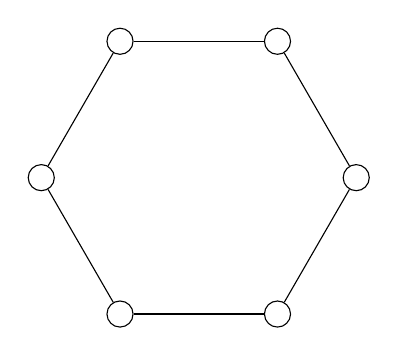
\begin{tikzpicture}
      % Draw the vertices
      \foreach \i in {1,2,3,4,5,6}
        \node[draw, circle] (\i) at ({60 * \i}:2) {};
    
      % Draw the edges
      \foreach \i/\j in {1/2, 2/3, 3/4, 4/5, 5/6, 6/1}
        \draw (\i) -- (\j);
    \end{tikzpicture}
    \item[(4)]  {3, 3, 3, 2, 2, 2} \\
    \textbf{Sum of degrees}: \( 3 + 3 + 3 + 2 + 2 + 2 = 15 \) (odd number). \\ 
    \textbf{Conclusion}: This sequence is \textbf{not graphic}, because the sum of the degrees is odd, violating the Handshaking Lemma.
    \item[(5)]  {3, 3, 2, 2, 2, 2} \\
    \textbf{Sum of degrees}: \( 3 + 3 + 2 + 2 + 2 + 2 = 14 \) (even number).\\
    \textbf{Havel-Hakimi check}:
    \begin{itemize}
        \item \( 3, 3, 2, 2, 2, 2 \)
        \item Remove a 3, subtract 1 from the next three: \( 2, 2, 1, 1, 2 \)
        \item Remove a 2, subtract 1 from the next two: \( 1, 1, 1, 1 \)
        \item Remove a 1, subtract 1 from the next one: \( 0, 0, 0 \).
    \end{itemize}
    \textbf{Conclusion}: This sequence is \textbf{graphic}. One possible graph is a 6-vertex cycle where alternating vertices have degree 3 and 2. \\
    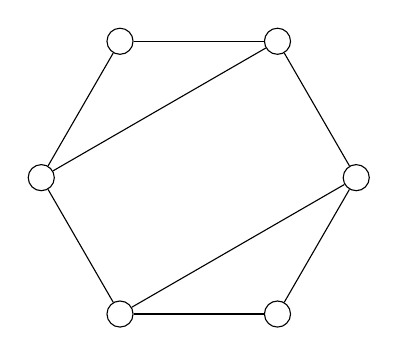
\begin{tikzpicture}
      % Draw the vertices
      \foreach \i in {1,2,3,4,5,6}
        \node[draw, circle] (\i) at ({60 * \i}:2) {};
    
      % Draw the edges (cycle)
      \foreach \i/\j in {1/2, 2/3, 3/4, 4/5, 5/6, 6/1}
        \draw (\i) -- (\j);
        
      % Additional edges to satisfy degree 3
      \draw (1) -- (3);
      \draw (4) -- (6);
    \end{tikzpicture}
    \item[(6)]  {1, 1, 1, 1, 1, 1} \\
    \textbf{Sum of degrees}: \( 1 + 1 + 1 + 1 + 1 + 1 = 6 \) (even number). \\
    \textbf{Havel-Hakimi check}:
    \begin{itemize}
        \item \( 1, 1, 1, 1, 1, 1 \)
        \item Remove a 1, subtract 1 from the next one: \( 0, 0, 0, 0, 0 \).
    \end{itemize}
    \textbf{Conclusion}: This sequence is \textbf{graphic}. The corresponding graph consists of 3 disjoint edges: \\    
    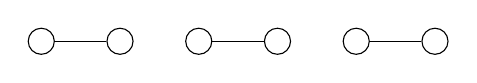
\begin{tikzpicture}
      % Draw the vertices
      \node[draw, circle] (A1) at (0,0) {};
      \node[draw, circle] (A2) at (1,0) {};
      \node[draw, circle] (B1) at (2,0) {};
      \node[draw, circle] (B2) at (3,0) {};
      \node[draw, circle] (C1) at (4,0) {};
      \node[draw, circle] (C2) at (5,0) {};
    
      % Draw the edges
      \draw (A1) -- (A2);
      \draw (B1) -- (B2);
      \draw (C1) -- (C2);
    \end{tikzpicture}
    \item[(7)]  {5, 3, 3, 3, 3, 3} \\
    \textbf{Sum of degrees}: \( 5 + 3 + 3 + 3 + 3 + 3 = 20 \) (even number). \\
    \textbf{Havel-Hakimi check}:
    \begin{itemize}
        \item \( 5, 3, 3, 3, 3, 3 \)
        \item Remove a 5, subtract 1 from the next five: \( 2, 2, 2, 2, 2 \)
        \item Remove a 2, subtract 1 from the next two: \( 1, 1, 1, 1 \)
        \item Remove a 1, subtract 1 from the next one: \( 0, 0, 0 \).
    \end{itemize}
    \textbf{Conclusion}: This sequence is \textbf{graphic}. One possible graph is a star graph with one vertex of degree 5: \\
    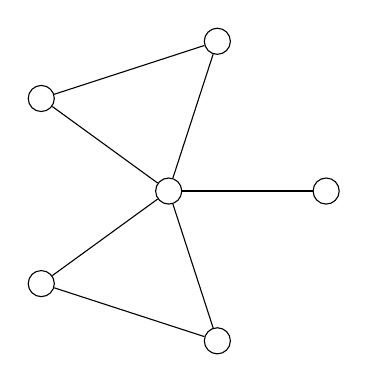
\begin{tikzpicture}
      % Draw the center vertex
      \node[draw, circle] (center) at (0,0) {};
    
      % Draw the outer vertices
      \foreach \i in {1,2,3,4,5}
        \node[draw, circle] (\i) at ({72 * \i}:2) {};
    
      % Draw edges from the center vertex to each outer vertex
      \foreach \i in {1,2,3,4,5}
        \draw (center) -- (\i);

      % Connect remaining vertices to match degree 3
      \draw (1) -- (2);
      \draw (3) -- (4);
    \end{tikzpicture}
    \item[(8)]  {5, 5, 4, 3, 2, 1} \\
    \textbf{Sum of degrees}: \( 5 + 5 + 4 + 3 + 2 + 1 = 20 \) (even number). \\
    \textbf{Havel-Hakimi check}:
    \begin{itemize}
        \item \( 5, 5, 4, 3, 2, 1 \)
        \item Remove a 5, subtract 1 from the next five: \( 4, 3, 2, 1, 0 \)
        \item Remove a 4, subtract 1 from the next four: \( 2, 1, 0, 0 \)
        \item Remove a 2, subtract 1 from the next two: \( 0, 0, 0 \).
    \end{itemize}
    \textbf{Conclusion}: This sequence is \textbf{graphic}. A possible graph satisfying the degree sequence is: \\
    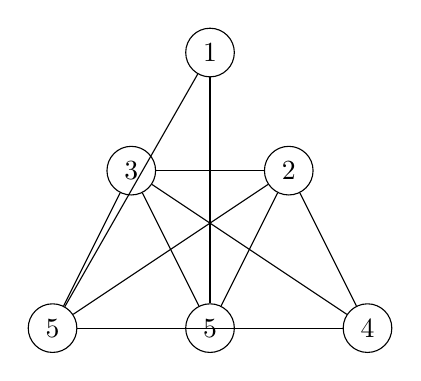
\begin{tikzpicture}
        % Draw vertices
        \node[draw, circle] (v1) at (0, 0) {5};
        \node[draw, circle] (v2) at (2, 0) {5};
        \node[draw, circle] (v3) at (4, 0) {4};
        \node[draw, circle] (v4) at (1, 2) {3};
        \node[draw, circle] (v5) at (3, 2) {2};
        \node[draw, circle] (v6) at (2, 3.5) {1};
        
        % Draw edges
        \draw (v1) -- (v2);
        \draw (v1) -- (v3);
        \draw (v1) -- (v4);
        \draw (v1) -- (v5);
        \draw (v1) -- (v6);
        
        \draw (v2) -- (v3);
        \draw (v2) -- (v4);
        \draw (v2) -- (v5);
        \draw (v2) -- (v6);
        
        \draw (v3) -- (v4);
        \draw (v3) -- (v5);
        \draw (v4) -- (v5);
    \end{tikzpicture}
\end{itemize}

\vs\
\end{itemize} 
 
\noindent{\bf Problem 2: } (10 points)
\vs\

A graph $G = (V, E)$, $|V|=n$, is bipartite if its vertices can be partitioned into two subsets $V = A \cup B$ such that all edges connect only vertices between the two sets (no two edges in the same set are connected).

Is the given statement True or False? If it is true, give a proof. If it is false, give a counter example.
\begin{itemize}
    \item[(a)] If a graph G is bipartite, then G is a tree. \\
    \textbf{Answer:} False. Not all bipartite graphs are trees. A counterexample is a 4-vertex cycle graph.
    \item[(b)] If a graph G is a tree, then it is bipartite. \\
    \textbf{Answer:} True. Every tree is bipartite.
    \begin{proof}
    Let \( G = (V, E) \) be a tree, which means \( G \) is a connected acyclic graph. We need to show that \( G \) is bipartite, i.e., that the vertex set \( V \) can be partitioned into two disjoint sets \( A \) and \( B \) such that every edge in \( E \) connects a vertex in \( A \) to a vertex in \( B \), with no edge connecting two vertices within the same set.
    \begin{enumerate}
        \item Start by choosing an arbitrary vertex \( v_0 \in V \) and perform a breadth-first search (BFS) or depth-first search (DFS) traversal starting from \( v_0 \). During the traversal, we will color the vertices in two colors, say \textbf{color red} and \textbf{color blue}, which correspond to the two sets \( A \) and \( B \) we are trying to construct.
        \item Assign vertex \( v_0 \) to set \( A \) (color red).
        \item For each vertex adjacent to \( v_0 \), assign it to set \( B \) (color blue). More generally, for any vertex that is reached during the traversal:
        \begin{itemize}
            \item If the vertex is assigned to set \( A \) (color red), assign all of its neighbors to set \( B \) (color blue).
            \item If the vertex is assigned to set \( B \) (color blue), assign all of its neighbors to set \( A \) (color red).
        \end{itemize}
        \item Continue this process for all vertices encountered during the traversal. Since \( G \) is a tree, it has no cycles, and this coloring scheme will not lead to any conflicts. Specifically, no two adjacent vertices will be assigned to the same set (i.e., both in \( A \) or both in \( B \)) because:
        \begin{itemize}
            \item Every time a vertex is colored, all of its neighbors are assigned the opposite color.
        \end{itemize}
        \item Since the graph is acyclic, we will not encounter any conflicts or contradictions during the traversal. In other words, there is no point in the process where an edge would connect two vertices in the same set.
    \end{enumerate}
    \noindent After coloring all the vertices of \( G \), we have successfully partitioned the vertex set \( V \) into two sets \( A \) and \( B \) such that every edge connects a vertex in \( A \) to a vertex in \( B \). Thus, the graph is bipartite.
    \textbf{Therefore,} every tree is bipartite.
    \end{proof}
\end{itemize}

\vs\

\newpage
\noindent{\bf Problem 3: } (10 points)
\vs\
Step through the following  BFS algorithm (CLRS textbook) for the following given graph with the starting vertex "A" and fill in the entries in the given table as shown in the class lecture. You need to show any intermediate values too.

\begin{algorithm}
\caption{BFS($G, s$)}
\begin{algorithmic}[1]
\For{each vertex $u \in G.V - \{s\}$}
    \State $u.color \gets \text{WHITE}$
    \State $u.d \gets \infty$
    \State $u.\pi \gets \text{NIL}$
\EndFor
\State $s.color \gets \text{GRAY}$
\State $s.d \gets 0$
\State $s.\pi \gets \text{NIL}$
\State $Q \gets \emptyset$
\State ENQUEUE($Q, s$)
\While{$Q \neq \emptyset$}
    \State $u \gets$ DEQUEUE($Q$)
    \For{each $v \in \text{Adj}[u]$}
        \If{$v.color == \text{WHITE}$}
            \State $v.color \gets \text{GRAY}$
            \State $v.d \gets u.d + 1$
            \State $v.\pi \gets u$
            \State ENQUEUE($Q, v$)
        \EndIf
    \EndFor
    \State $u.color \gets \text{BLACK}$
\EndWhile
\end{algorithmic}
\end{algorithm}

\begin{figure}[!h]
\centering
\includegraphics[scale=.74]{graph-image-v1.jpg}
\end{figure}


\begin{tabular}{|c|c|c|c|} \hline
  Vertex  & \hs\ \ha\  Color \hs\ \ha\ & \hs\  Distance \hs\ & \ha\ Predecessor \ha\  \\
  $v$ & $v.color$ & $v.d$ & $v.\pi$ \\ \hline
  A & & & \\ \hline
  B & & & \\ \hline
  C & & & \\ \hline
  D & & & \\ \hline
  E & & & \\ \hline
  F & & & \\ \hline
  G & & & \\ \hline
  H & & & \\ \hline
  I & & & \\ \hline
\end{tabular} \\

\textbf{Answer:}

\begin{tabular}{|c|c|c|c|} \hline
  Vertex  & \hs\ \ha\  Color \hs\ \ha\ & \hs\  Distance \hs\ & \ha\ Predecessor \ha\  \\ \hline
  A & GRAY & 0 & Nil \\ \hline
  B & GRAY & 1 & A \\ \hline
  C & WHITE & $\infty$ & Nil \\ \hline
  D & WHITE & $\infty$ & Nil \\ \hline
  E & WHITE & $\infty$ & Nil \\ \hline
  F & WHITE & $\infty$ & Nil \\ \hline
  G & WHITE & $\infty$ & Nil \\ \hline
  H & GRAY & 1 & A \\ \hline
  I & WHITE & $\infty$ & Nil \\ \hline
\end{tabular}
\vs\

\noindent{After processing B:}

\begin{tabular}{|c|c|c|c|} \hline
  Vertex  & \hs\ \ha\  Color \hs\ \ha\ & \hs\  Distance \hs\ & \ha\ Predecessor \ha\  \\ \hline
  A & BLACK & 0 & Nil \\ \hline
  B & BLACK & 1 & A \\ \hline
  C & GRAY & 2 & B \\ \hline
  D & WHITE & $\infty$ & Nil \\ \hline
  E & WHITE & $\infty$ & Nil \\ \hline
  F & WHITE & $\infty$ & Nil \\ \hline
  G & WHITE & $\infty$ & Nil \\ \hline
  H & GRAY & 1 & A \\ \hline
  I & WHITE & $\infty$ & Nil \\ \hline
\end{tabular}
\vs\

\noindent{After processing H:}

\begin{tabular}{|c|c|c|c|} \hline
  Vertex  & \hs\ \ha\  Color \hs\ \ha\ & \hs\  Distance \hs\ & \ha\ Predecessor \ha\  \\ \hline
  A & BLACK & 0 & Nil \\ \hline
  B & BLACK & 1 & A \\ \hline
  C & GRAY & 2 & B \\ \hline
  D & WHITE & $\infty$ & Nil \\ \hline
  E & WHITE & $\infty$ & Nil \\ \hline
  F & WHITE & $\infty$ & Nil \\ \hline
  G & GRAY & 2 & H \\ \hline
  H & BLACK & 1 & A \\ \hline
  I & GRAY & 2 & H \\ \hline
\end{tabular}
\vs\

\noindent{After processing C:}

\begin{tabular}{|c|c|c|c|} \hline
  Vertex  & \hs\ \ha\  Color \hs\ \ha\ & \hs\  Distance \hs\ & \ha\ Predecessor \ha\  \\ \hline
  A & BLACK & 0 & Nil \\ \hline
  B & BLACK & 1 & A \\ \hline
  C & BLACK & 2 & B \\ \hline
  D & WHITE & $\infty$ & Nil \\ \hline
  E & WHITE & $\infty$ & Nil \\ \hline
  F & WHITE & $\infty$ & Nil \\ \hline
  G & GRAY & 2 & H \\ \hline
  H & BLACK & 1 & A \\ \hline
  I & GRAY & 2 & H \\ \hline
\end{tabular}
\vs\

\noindent{After processing G:}

\begin{tabular}{|c|c|c|c|} \hline
  Vertex  & \hs\ \ha\  Color \hs\ \ha\ & \hs\  Distance \hs\ & \ha\ Predecessor \ha\  \\ \hline
  A & BLACK & 0 & Nil \\ \hline
  B & BLACK & 1 & A \\ \hline
  C & BLACK & 2 & B \\ \hline
  D & WHITE & $\infty$ & Nil \\ \hline
  E & WHITE & $\infty$ & Nil \\ \hline
  F & GRAY & 3 & G \\ \hline
  G & BLACK & 2 & H \\ \hline
  H & BLACK & 1 & A \\ \hline
  I & GRAY & 2 & H \\ \hline
\end{tabular}
\vs\

\noindent{After processing I:}

\begin{tabular}{|c|c|c|c|} \hline
  Vertex  & \hs\ \ha\  Color \hs\ \ha\ & \hs\  Distance \hs\ & \ha\ Predecessor \ha\  \\ \hline
  A & BLACK & 0 & Nil \\ \hline
  B & BLACK & 1 & A \\ \hline
  C & BLACK & 2 & B \\ \hline
  D & GRAY & 3 & I \\ \hline
  E & WHITE & $\infty$ & Nil \\ \hline
  F & GRAY & 3 & G \\ \hline
  G & BLACK & 2 & H \\ \hline
  H & BLACK & 1 & A \\ \hline
  I & BLACK & 2 & H \\ \hline
\end{tabular}
\vs\

\noindent{After processing F:}

\begin{tabular}{|c|c|c|c|} \hline
  Vertex  & \hs\ \ha\  Color \hs\ \ha\ & \hs\  Distance \hs\ & \ha\ Predecessor \ha\  \\ \hline
  A & BLACK & 0 & Nil \\ \hline
  B & BLACK & 1 & A \\ \hline
  C & BLACK & 2 & B \\ \hline
  D & GRAY & 3 & I \\ \hline
  E & GRAY & 4 & F \\ \hline
  F & BLACK & 3 & G \\ \hline
  G & BLACK & 2 & H \\ \hline
  H & BLACK & 1 & A \\ \hline
  I & BLACK & 2 & H \\ \hline
\end{tabular}
\vs\

\noindent{After processing D:}

\begin{tabular}{|c|c|c|c|} \hline
  Vertex  & \hs\ \ha\  Color \hs\ \ha\ & \hs\  Distance \hs\ & \ha\ Predecessor \ha\  \\ \hline
  A & BLACK & 0 & Nil \\ \hline
  B & BLACK & 1 & A \\ \hline
  C & BLACK & 2 & B \\ \hline
  D & BLACK & 3 & I \\ \hline
  E & GRAY & 4 & F \\ \hline
  F & BLACK & 3 & G \\ \hline
  G & BLACK & 2 & H \\ \hline
  H & BLACK & 1 & A \\ \hline
  I & BLACK & 2 & H \\ \hline
\end{tabular}
\vs\

\noindent{After processing E:}

\begin{tabular}{|c|c|c|c|} \hline
  Vertex  & \hs\ \ha\  Color \hs\ \ha\ & \hs\  Distance \hs\ & \ha\ Predecessor \ha\  \\ \hline
  A & BLACK & 0 & Nil \\ \hline
  B & BLACK & 1 & A \\ \hline
  C & BLACK & 2 & B \\ \hline
  D & BLACK & 3 & I \\ \hline
  E & BLACK & 4 & F \\ \hline
  F & BLACK & 3 & G \\ \hline
  G & BLACK & 2 & H \\ \hline
  H & BLACK & 1 & A \\ \hline
  I & BLACK & 2 & H \\ \hline
\end{tabular}


\vs\
\ls\

\end{document}